%!TEX TS-program = xelatex
%!TEX encoding = UTF-8 Unicode

\documentclass[nols,b5paper]{tufte-book}

\usepackage{booktabs}
\usepackage{graphicx}
\usepackage{listings}

\usepackage{mathspec}
\usepackage{fontspec,xltxtra,xunicode}
\defaultfontfeatures{Mapping=tex-text}
\setromanfont[Mapping=tex-text]{Warnock Pro Light}
\setsansfont[Scale=MatchLowercase,Mapping=tex-text]{Frutiger LT Std}
\setmonofont[Scale=MatchLowercase]{Andale Mono}
\setmathfont(Greek,Latin,Digits){Warnock Pro Light}

\graphicspath{{./figures/}}

\usepackage{color}
\lstset{
         basicstyle=\footnotesize\ttfamily, % Standardschrift
         numbers=left,               % Ort der Zeilennummern
         numberstyle=\tiny,          % Stil der Zeilennummern
         %stepnumber=2,               % Abstand zwischen den Zeilennummern
         numbersep=5pt,              % Abstand der Nummern zum Text
         tabsize=2,                  % Groesse von Tabs
         extendedchars=true,         %
         breaklines=true,            % Zeilen werden Umgebrochen
         keywordstyle=\color{red},
    	 frame=b,         
         stringstyle=\color{white}\ttfamily,
         showspaces=false,
         showtabs=false,
         xleftmargin=17pt,
         framexleftmargin=17pt,
         framexrightmargin=5pt,
         framexbottommargin=4pt,
         %backgroundcolor=\color{lightgray},
         showstringspaces=false
 }

\lstloadlanguages{Python}
\usepackage{caption}
\DeclareCaptionFont{white}{\color{white}}
\DeclareCaptionFormat{listing}{\colorbox[cmyk]{0.43, 0.35, 0.35,0.01}{\parbox{\textwidth}{\hspace{15pt}#1#2#3}}}
\captionsetup[lstlisting]{format=listing,labelfont=white,textfont=white, singlelinecheck=false, margin=0pt, font={bf,footnotesize}}


\title[\textsc{bipy user manual}]{bipy user manual}
\author[\textsc{Timothée Poisot}]{Timothée Poisot}
\date{Version pre 1.0}

\begin{document}

\maketitle
\tableofcontents

\chapter{Introduction}

\texttt{bipy} is a set of functions written in Python, whose goal is to make it easy to analyze and visualize bipartite networks. This document describes the use of the \texttt{bipy}. This documentation is valid only for the versions before the 1.0 release (scheduled to occur sometime in the fall or winter of 2011). The aim of this documentation is to present only the ``high-level'' functions, i.e. these that the user will need to perform the analyses (although \texttt{bipy} was conceived to automate most of the analyses, so there are a very small number of functions that need to be known). In addition, some background about the measures used and the most important references will be given.

This guide should be viewed as a quick walkthrough to the features, and is intended primarily for the people that want to analyze their data without spending much effort in understanding the mechanisms behind the analyses. The ``\nameref{c:ex}'' on p. \pageref{c:ex} gives some complete scripts to perform the most common analyses.

\subsection{Installing \texttt{bipy}}

\texttt{bipy} can be obtained on \emph{GitHub} (http://github.com/tpoisot/bipy). There are a number of required additional software. Obviously, \texttt{bipy} requires a Python installation, preferentially 2.6 or 2.7. For those of you with a Mac, you need to download the version from python.org (http://www.python.org/getit/).

Once this is done, 

\subsection{Do I need to know Python ?}

This is a good question! If you just want to have basic informations about your data, the short answer is \textbf{no}. \texttt{bipy} was designed from the beginning to automate most of the calculations, and use the most robust statistics available, so you don't have to play too much with the code. Most of what you will have to do is start python, load your data, and use the summary functions.

If you want to use \texttt{bipy} for more complicated analyses, then \textbf{yes}, learning python will definitely be a huge plus. But if you are willing to adopt a computational approach, chances are you already know a programming language, and you should be able to pick up python really quick.

\subsection{How do I cite \texttt{bipy} ?}

For the moment, just cite (by replacing the date with the day you downloaded it):

\begin{quote}
	Poisot, T. (2011) \texttt{bipy} -- bipartite networks analysis using python. http://github.com/tpoisot/bipy. Downloaded on \today.
\end{quote}

A paper formally describing \texttt{bipy} (along with alternatives in other languages) is currently being written.

\chapter{Loading data}

This chapter describes how to load data in a format that can be understood by \texttt{bipy}. There are two different ways to load data in \texttt{bipy}: \emph{via} a text file, or \emph{via} the web \footnote{Actually, there exists a third way to load data, namely the interaction with the \textsc{ewdb} -- given that this database is still highly experimental, and that the server on which it is developed is not ready to support real usage, this will be introduced in future versions of \texttt{bipy}. }. We will cover both in this chapter.

\subsection{What should the data look like ?}

\texttt{bipy} assumes that a bipartite network is nothing more than a matrix, in which each square represents the strength of the interaction between a species from the top trophic level, and a species from the bottom trophic level. Thus, a bipartite network is defined by a matrix $\mathbf{M}$, in which $\mathbf{M}\sb{ij}$ is the strength of the link between upper trophic level species $i$ and lower trophic level species $j$. It is assumed that the rows of $\mathbf{M}$ are the upper trophic level species. This is a notational convention, but we will stick to it through all the documentation.

The advantage of this organization of the data is that it can easily be stored in a text file, with each interaction strength separated by a space, and the different organisms separated by a new line. Thus, the file

\begin{marginfigure}[3cm]
	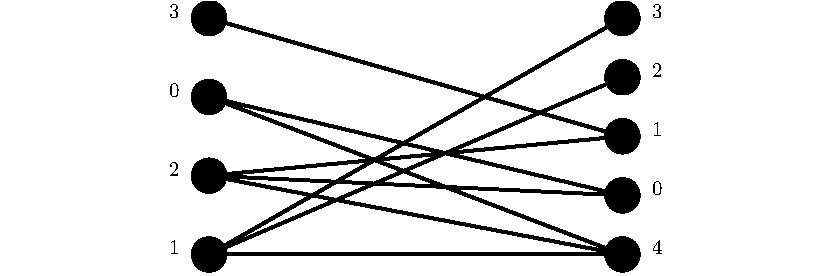
\includegraphics[width=4.5cm]{ex-1}
\end{marginfigure}

\begin{verbatim}
1 0 0 0 1
0 0 1 1 1
1 1 0 0 1
0 1 0 0 0
\end{verbatim}

\noindent described the network illustrated in the margin. Of course, the values within the file can be anything (as long as they are numeric): zeroes and ones, number of visits, predation rate, percent of the diet, and so on.

However, an interaction network is much more than the interaction matrix. When an interaction matrix is loaded, \texttt{bipy} will automatically initiate the calculation of several important metrics. This has two advantages. First, these metrics are needed for multiple calculations, so instead of being re-calculated several times, they are calculated only once. This speeds-up calculation time. Second, the object is easier to manipulate, as it keeps all the relevant informations together. For example, the connectance of a \texttt{bipartite} object called \texttt{w} is \texttt{w.connectance}.

Loading data will read the interaction matrix, and generate this \texttt{bipartite} object, which will be used in nearly all the analyses after. This requires no input from the user, so getting the data ready to work is really straightforward.

\subsection{Reading data from a local file}

Assuming that your data are in this format, and the file is called \texttt{mydata.web}, you can load them

\begin{lstlisting}[caption=loading data from a file]
web = loadweb('mydata.web')
\end{lstlisting}

At this point, the most difficult part is done. Your data are loaded, and you will be able to see what story they tell using the metrics described in the other chapters.

If your data are not in the ``correct'' format, i.e. the top level organisms are in columns, do not panic. You just need to pass a supplementary argument \texttt{t} to the \texttt{loadweb} function:

\begin{lstlisting}[caption=loading data from a file and transposing the data]
web = loadweb('mydata.web',t=True)
\end{lstlisting}

This will tell \texttt{bipy} that your data need to be transposed before going on with the analysis. For a non-console version, just use \texttt{loadweb} with no parameters (you can still specificity \texttt{t=True} if you want to transpose your data):

\begin{lstlisting}[caption=opening a file dialog]
web = loadweb()
\end{lstlisting}

\texttt{loadweb} will open the file selection dialog of your operating system, so you can pick your dataset.

\subsection{Reading data from the web}

The alternative way is to load data stored on the internet. \texttt{bipy} is able to do so by using the \texttt{readRemoteWeb} function, which requires two arguments. The first one is the \textsc{url} of a text file, which stores the interaction matrix. The second tells if the network should be transposed (false by default).

\begin{lstlisting}[caption=reading a dataset from the web]
web = readRemoteWeb('http://server/mydata.web'),False)
\end{lstlisting}

This method can be used to load networks made publicly available on the \textsc{iwdb} (http://www.nceas.ucsb.edu/interactionweb/), for example.

\subsection{Adding species names}

\texttt{bipy} has the ability to store the names of the species in the network. Currently, the way to do it is to assign a value to the properties \texttt{lonames} and \texttt{upnames} of a \texttt{bipartite} object. An easier way to load the data is currently being implemented.

The code to assign species names is:

\begin{lstlisting}[caption=attributing species names]
web = bipartite(readweb('mydata.web'))
web.lonames = ['plant1','plant2','plant3',...]
web.upnames = ['herb1','herb2','herb3',...]
\end{lstlisting}

\texttt{bipy} internally takes care of re-ordering the species names when the matrix is sorted (to reflect nestedness or modularity). In addition, the species names are used in some visualizations, and when generating species-level metrics summaries. 

\subsection{Adding bibliographical references}

When comparing several datasets, it may be interesting to know where the data come from. \texttt{bipy} is able to extract bibliographic information from several identifiers, and to generate a link to the original paper.

If you have a dataset loaded, you can add the original references and see them by doing:

\begin{lstlisting}[caption=attributing a reference]
web.ref = ref({'doi':'10.1098/rsbl.2010.0774,'pmid':'20961886'})})
output_citinfo(w)
\end{lstlisting}

This uses some \textsc{ncbi} functions to get the original data, so you need to be online to use it. 

\chapter{Species--level metrics}

\chapter{Network--level metrics}

\chapter{Null models}

\chapter{Graphics}

\texttt{bipy} comes with several ways to visualize the data, which are meant to reflect the properties of the networks.

\chapter{Example scripts\label{c:ex}}

\end{document}